\section{Random Processes and Monte-Carlo Methods}
\subsection{Random Number Genarators}
The discussed equations produce seemingly random numbers given a seed number. However, these aren't truly random as they are deterministic and can be re-discovered given the seed number is known. Hence, they are referred to as \textbf{pseudorandom numbers.}
\par 
Consider the equation:
$$x^{\prime}=(ax+c) mod (m), $$
where $a,c,m$ are integer constants and $x$ is an integer variable. Given a value of $x$ (seed), $x^{\prime}$ is the resultant integer which can be re-fed to the equation as $x$. This is a \textit{linear congruential random number genarator.}
\subsection{Radioactive Decay Chain}
$^{213}Bi$ deacays to stable $^{209}Bi$ via two different routes given as:

\begin{center}


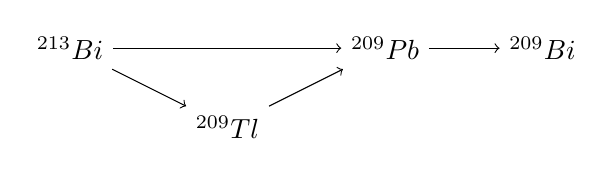
\begin{tikzpicture}[node distance=2cm][H]
% nodes

\node (A) at (0, 0) {$^{213}Bi$};
\node (B) at (2,-1 ) {$^{209}Tl$};
\node (C) at (4,0 ) {$^{209}Pb$};
\node (D) at (6,0 ) {$^{209}Bi$};


% arrows
\draw [->] (A)--(B);
\draw [->] (B)--(C);
\draw [->] (A)--(C);
\draw [->] (C)--(D);

\end{tikzpicture}
\end{center}
Here, we begin with $10,000$ atoms of $^{213}Bi$ and for each such atom, we generate a random number between $0$ and $1$. We, compare the number with the probability of the decay of such an atom in time $t$ which is given by the equation:
$$p(t)=1-2^{-\dfrac{t}{\tau}},
$$
where $\tau$ is the half-life for $^{213}Bi$. We calculate the probability for $t=1 sec$ with $t_{max}=20,000 seconds$. This is done for all decaying entities, namely, $^{213}Bi$, $^{209}Tl$,  and  $^{209}Pb$
\begin{lstlisting}[language=Python, caption=Decay Chain, frame=single, label={lst:decay} ]
Bi213=10000
Tl=0
Pb=0
Bi209=0
tau1=46*60
tau2=2.2*60
tau3=3.3*60
h=1
p1=1-2**(-h/tau1)
p2=1-2**(-h/tau2)
p3=1-2**(-h/tau3)
tmax=20000
b2p=0.9791
b2t=1-b2p
NTl=[]
NPb=[]
NBi213=[]
NBi209=[]
tpoints=np.arange(0,tmax,h)
for t in tpoints:
	Pbdecay=0
	Bi213decay=0
	Tldecay=0
	for p in range(Pb):
		if np.random.rand()<p3:
			Pbdecay+=1
	for t in range(Tl):
		if np.random.rand()<p2:
			Tldecay+=1
	for b in range(Bi213):
		if np.random.rand()<p1:
			Bi213decay+=1

	Pb-=Pbdecay
	Bi209+=Pbdecay
	Pb+=Tldecay
	Tl-=Tldecay
	Bi213-=Bi213decay
	b2pdecay=0
	b2tdecay=0
	for _ in range(Bi213decay):
		if np.random.rand()<b2p:
			b2pdecay+=1
		else:
			b2tdecay+=1
	Pb+=b2pdecay
	Tl+=b2tdecay

	NTl.append(Tl)
	NPb.append(Pb)
	NBi213.append(Bi213)
	NBi209.append(Bi209)


\end{lstlisting}
\begin{figure}[H]
	\centering
	\includegraphics[width=0.7\linewidth]{../../../Images/RadioactiveDecay}
	\caption{Decay Graph}
	\label{fig:radioactivedecay}
\end{figure}
\subsection{Brownian Motion}
To simulate a random walk, I assume a Canvas of size $500*500$ pixels. We select at random, one of 4 directions : Up, Down, Left, and Right. Running the code for some prescribed number of iterations $N$, we obtain random paths. The code is as follows:
\begin{lstlisting}[language=Python, caption=Random Walk, frame=single, label={lst:randomwalk} ]
N=100000*3
current_pos=np.array([250,250])
canvas=np.zeros([501,501])
def fill(Dir, current_pos):
	x,y=current_pos
	if Dir==0:
		dx,dy=-1,0
	if Dir==1:
		dx,dy=+1,0
	if Dir==2:
		dx,dy=0,+1
	if Dir==3:
		dx,dy=0,-1
	if (x+dx)<0 or (x+dx)>500:
		dx=0
	if (y+dy)<0 or (y+dy)>500:
		dy=0
	canvas[x+dx,y+dy]+=1
	return np.array([x+dx,y+dy])
for i in range(N):
	Dir=np.random.randint(4)
	current_pos=fill(Dir, current_pos)
plt.imshow(canvas)

\end{lstlisting}
\begin{figure}[H]
	\centering
	\includegraphics[width=0.7\linewidth]{../../../Images/RandomWalk}
	\caption[Random Walk]{Random Walk: Output for Above Code}
	\label{fig:randomwalk}
\end{figure}
\subsection{Monte-Carlo Integration}
To integrate a function $f(x)$ in range $[a,b]$, with the maximum and minimum values $f_{max}$ and $f_{min}$, consider a rectangle enclosing the function, having area $A$. We choose at random, points inside the rectangle and check whether they fall within the area of the function. Then, the probability that a given point lies in the area is given $I\div A$. Let the probability be $P=K \div N$, where $K$ is number of points that fall within the area and $N$ is total number of points. Hence,
$$I \approx \dfrac{K*A}{N}$$
Following code outlines the way to obtain an integral for the function:
$$f(x) = \sin^{2} \left(\dfrac{1}{x*(2-x)}\right),$$ in range $[0,2]$
\begin{lstlisting}[language=Python, caption=Monte Carlo Integration, frame=single, label={lst:montecarlo} ]
def f(x):
	return (np.sin(1/(x*(2-x))))**2
N=10000
count=0
A=2
for i in range(N):
	x=2*random.rand()
	y=random.rand()
	if y<f(x):
		count+=1
print(A*count/N)
\end{lstlisting}
\begin{figure}[H]
	\centering
	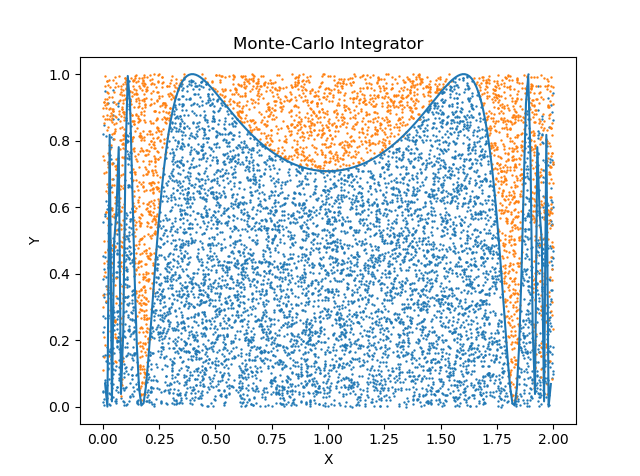
\includegraphics[width=0.7\linewidth]{MonteCarlo}
	\caption{Random Points used to calculate Integral}
	\label{fig:montecarlo}
\end{figure}
\subsection{Mean Value Method}
The average value of $f(x)$ in range from $a$ to $b$ is by definition:
$$\braket{f}= \dfrac{1}{b-a}\int_{a}^{b}f(x)dx=\dfrac{I}{b-a}$$
Thus, $$I = (b-a)\braket{f}$$
A simple way to estimate $\braket{f}$ is to measure $f(x)$ at $N$ points, chosen uniformly at random between $a$ and $b$. Then,
$$I \approx \dfrac{b-a}{N}\sum_{i=1}^{N}f(x_{i})$$




